\documentclass{standalone}
\usepackage{tikz}
\usepackage{ctex,siunitx}
\setCJKmainfont{Noto Serif CJK SC}
\usepackage{tkz-euclide}
\usepackage{amsmath}
\usetikzlibrary{patterns, calc,3d}
\usetikzlibrary {decorations.pathmorphing,decorations.pathreplacing,decorations.shapes}
\begin{document}
\small
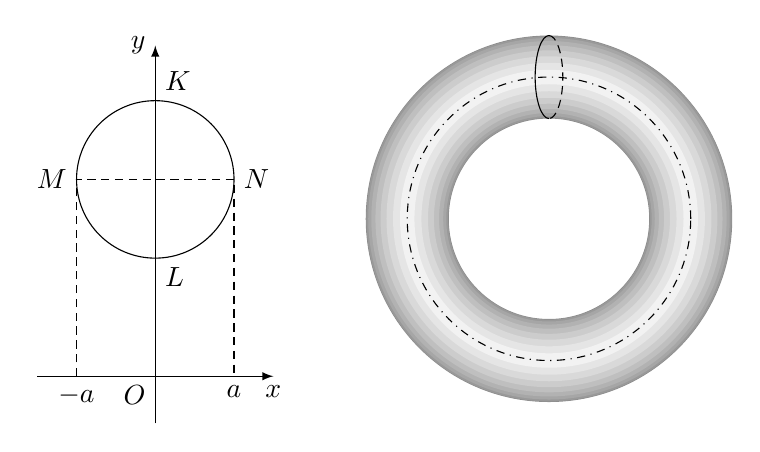
\begin{tikzpicture}[>=latex,scale=1.0]
  \draw[->](-1.5,0)--(1.5,0)node[below]{$x$};
  \draw[->](0,-0.6)--(0,4.2)node[left]{$y$};
  \node at (0,0)[below left]{$O$};
  \draw(0,2.5)circle(1);
  \draw[densely dashed](-1,0)node[below]{$-a$}--(-1,2.5)node[left]{$M$}--(1,2.5)node[right]{$N$}--(1,0)node[below]{$a$};
  \node at (0,3.5)[above right]{$K$};
  \node at (0,1.5)[below right]{$L$};
  \begin{scope}[xshift=5cm,yshift=2.0cm]
    \foreach \x in {90,80,...,10}
    {
      \draw[line width={30*sin(\x)},gray!\x](0,0)circle(1.8);
    }
    \draw[dashdotted](0,0)circle(1.8);
    \draw[densely dashed](90:1.8cm+15pt)arc(90:-90:5pt and 15pt);
    \draw(90:1.8cm+15pt)arc(90:270:5pt and 15pt);
  \end{scope}
\end{tikzpicture}
\end{document}